\documentclass[usenames, dvipsnames, t]{beamer}

%\usepackage{geometry}
%\geometry{legalpaper, textwidth=426pt}
%\usepackage[T1]{fontenc}
%\usepackage{fourier}
\usepackage{graphicx}
%\graphicspath{{Figures/}}
%
\usepackage[english]{babel}															% English language/hyphenation
%\usepackage[protrusion=true,expansion=true]{microtype}
\usepackage{amsmath,amsfonts,amsthm} % Math packages
\usefonttheme[onlymath]{serif}
\usepackage{graphicx, adjustbox}
\graphicspath{{figures/}}
%\usepackage{url}
\newcommand{\red}[1]{\textcolor{red}{#1}}
%
%% Self included packages
%%\usepackage[labelfont=sf,			hypcap=false,			format=hang,			width=\columnwidth]{caption}
%\usepackage{amsmath}
%\usepackage{wrapfig}
\usepackage[ruled, vlined]{algorithm2e}
\usepackage{pgfplots}
%\pgfplotsset{soldot/.style={color=blue,only marks,mark=*}} \pgfplotsset{holdot/.style={color=blue,fill=white,only marks,mark=*}}
\pgfplotsset{compat=1.12}
\usepackage{xcolor}
\usepackage{tikz}
\usetikzlibrary{graphs, graphs.standard, shapes.misc, positioning, fit, shadows, calc, snakes, shapes, patterns, arrows.meta, matrix, shapes.geometric}
% \usepackage[noend]{algpseudocode}
\usepackage{hyperref}
\hypersetup{
    colorlinks,
    citecolor=black,
    filecolor=black,
    linkcolor=black,
    urlcolor=black
}
%\usepackage{ifthen}
\usepackage{bm}
%\usepackage{enumerate}
%%%%%%%%%%%%%%%%%%%%%%%%%%%%%%%%%%%%%%%%%%%%%%%%%%%%%%%%%%%%%%%%%%%%%%%%%%%
\usetheme{CambridgeUS}
\usecolortheme{beaver}
\usepackage[english]{babel}

\setbeamertemplate{section in toc}{\inserttocsection}
\setbeamertemplate{subsection in toc}{\hspace{1.2em}~\inserttocsubsection\par}

\setbeamerfont{section in toc}{size=\small}
\setbeamerfont{subsection in toc}{size=\footnotesize}

\setbeamertemplate{itemize item}{\color{red}$\circ$}
\setbeamertemplate{itemize subitem}{\color{red}$\circ$}

\setbeamertemplate{enumerate item}[default]
\setbeamercolor*{enumerate item}{fg=red}
\setbeamercolor*{enumerate subitem}{fg=red}
\setbeamercolor*{enumerate subsubitem}{fg=red}

\setbeamertemplate{footline}
{
  \leavevmode%
  \hbox{%
  \begin{beamercolorbox}[wd=.2\paperwidth,ht=2.25ex,dp=1ex,center]{author in head/foot}%
  	\usebeamerfont{author in head/foot}\insertshortauthor
  \end{beamercolorbox}%

  \begin{beamercolorbox}[wd=.5\paperwidth,ht=2.25ex,dp=1ex,center]{title in head/foot}%
    	\usebeamerfont{title in head/foot}\insertshorttitle\hspace*{3em}
  \end{beamercolorbox}%

  \begin{beamercolorbox}[wd=.3\paperwidth,ht=2.25ex,dp=1ex,right]{date in head/foot}%
    	\usebeamerfont{date in head/foot}\insertshortdate{}\hspace*{2em}
	\insertframenumber{} / \inserttotalframenumber\hspace*{2ex}
  \end{beamercolorbox}}%
  \vskip0pt%
}

\title{DiffSim }
\subtitle{}
\author{Ludwig Winkler}
\institute{Machine Learning Group \\ TU Berlin}
\date{\today}


%%%%%%%%%%%%%%%%%%%%%%%%%%%%%%%%%%%%%%%%%%%%%%%%%%%%%%%%%%%%%%%%%%%%%%%%%%%%
\begin{document}

\def\mathn#1{\mathnormal{#1}}
\def\thet{\bm{\theta}}
\def\V{\mathn{V}}
\def\Q{\mathn{Q}}
\def\R{\mathn{R}}
\def\r{\mathn{r}}
\def\G{\mathn{G}}
\def\n{\mathn{n}}
\def\A{\mathn{A}}
\def\T{\mathn{T}}
\def\W{\mathn{W}}
% \def\E{\mathbb{E}}

\def\w{\mathn{w}}
\def\p{\mathn{p}}
\def\q{\mathn{q}}
\def\a{\mathn{a}}
\def\r{\mathn{r}}
\def\s{\mathn{s}}
\def\t{\mathn{t}}
\def\dist{1}

\newcommand{\E}{\mathbb{E}}

\tikzset{ shorten <>/.style={ shorten >=#1, shorten <=#1 } }


\begin{frame}
	\titlepage
\end{frame}

% \begin{frame}
% \frametitle{Outline}
% \tableofcontents
% \end{frame}

\begin{frame}
	\frametitle{DiffSim - Idea}
	\begin{itemize}
		\item Autodiff frameworks work great for machine learning: we compute gradients for parameters conveniently
		\item Why stop at computing parameter gradients? Why not autodiff arbitrary code?
		\item Big part of modern engineering/research are based on computer models/simulations
		\item[]
		\item Let's autodiff entire computer models/simulations!
		\item Question: What could we do with that?
	\end{itemize}
\end{frame}

\begin{frame}
	\frametitle{What's happened so far}
	\begin{itemize}
		\item Simulation of explicit high-dim simulation vs low-dim latent simulation [Rotating Gaussian distribution]
		\item Parts of latent simulation is done by neural network ODE
		\item[] 
		\item Chaotic system with external force field [Double Pendulum]
		\item[] 
		\item Three Body Problem of rotating planets [N-Body Problem]
	\end{itemize}
\end{frame}

\begin{frame}
	\frametitle{What's to discuss}
	\framesubtitle{Energy Conservation}
	\begin{itemize}
		\item Continuously adding an external force field massivily increases the energy of the system in the long run, aka erratic evolution
		\item I have to pay very close attention to how I design the noise force fields
		\item []
		\item Obvious solution: time varying, but I realized that too late as an explicit solution to this problem
		\item Wanted to work on time dependent DiffEqs anyway
	\end{itemize}
\end{frame}

\begin{frame}
	\frametitle{What's to discuss}
	\framesubtitle{N-dimensional Hamiltonian benchmark}
	\begin{itemize}
		\item Current benchmarks are unintuitive to debug
		\item More explicit state space debugging instead of human readable image space
		\item []
		\item Implement very high Hamiltonian system via GMM in 10-20 dimensions
		\item Visualize 2D trajectories from that high dimensional space
	\end{itemize}
\end{frame}

\begin{frame}
	\frametitle{What's to discuss}
	\framesubtitle{Visualization of Learnable Force Field}
	\begin{itemize}
		\item Lyapunov instability is annoying, since visualizations diverge long term ... but ...
	\end{itemize}
	\centering
	\begin{figure}
	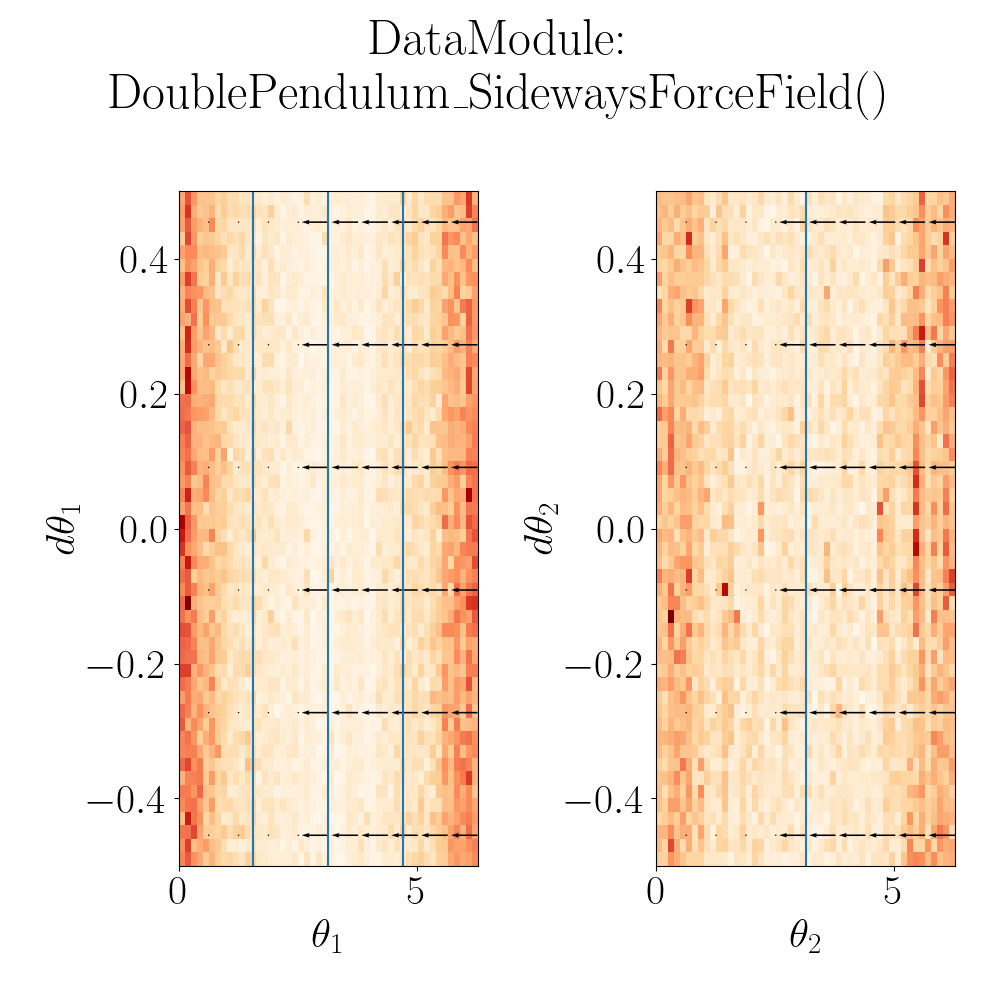
\includegraphics[height=0.7\textheight]{myplot1.png} 
	\end{figure}
\end{frame}

\begin{frame}
	\frametitle{What's to discuss}
	\framesubtitle{Visualization of Learnable Force Field}
	\begin{itemize}
		\item ... but Force Fields are explicitely learnable, color grading is training data distribution, but maybe only learns constant offset?
	\end{itemize}
	\centering
	\begin{figure}
	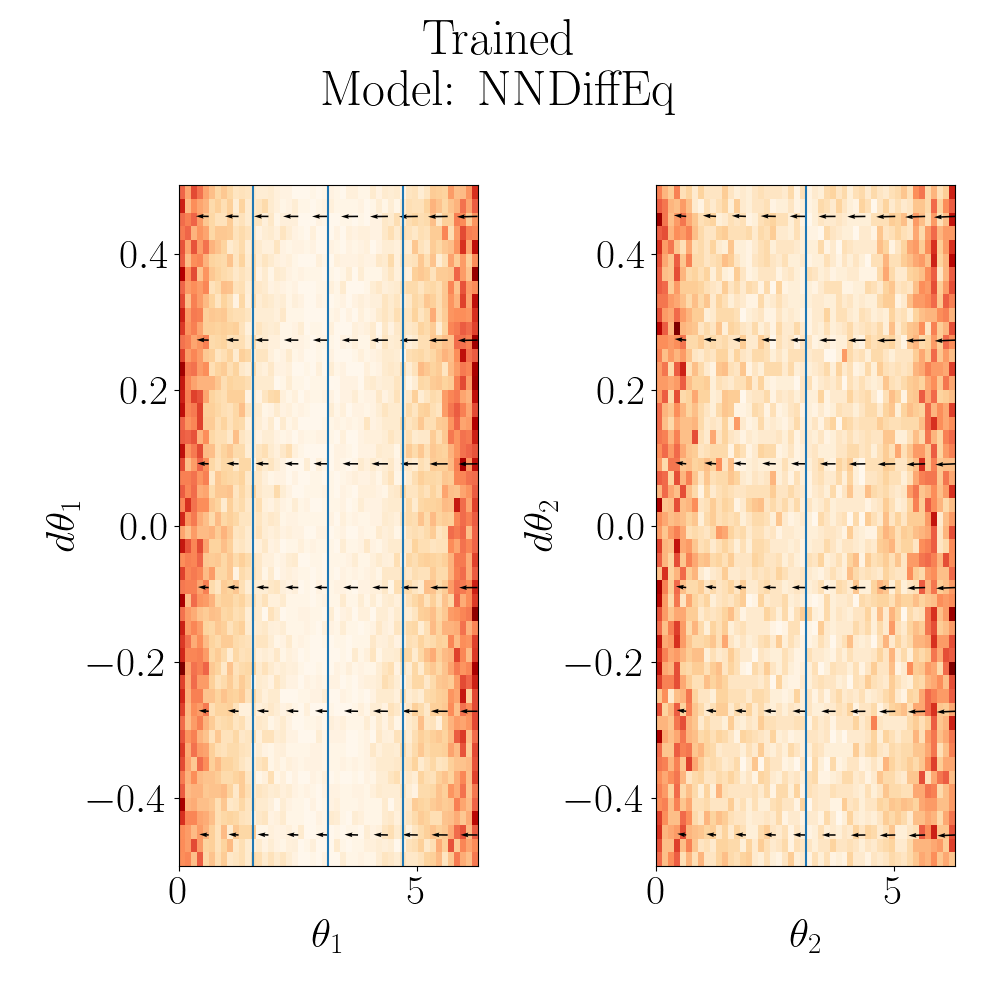
\includegraphics[height=0.7\textheight]{myplot.png} 
	\end{figure}
\end{frame}

\begin{frame}
	\frametitle{Next Step}
	\begin{itemize}
		\item Implement time dependent/varying DiffEqs 
		\item Devise energy stable noise force field development
		\item Hopefully use Nd Hamiltonian as well behaved benchmark to test out time dependent noise force fields
		\item With time dependent force fields, adding and subtracting energy is possible
		\item Implement N-dimensional Hamiltonian system to analyse sub trajectories
		\item[] 
	\end{itemize}
\end{frame}




\end{document}
